\newpage

\subsection*{Question 3}

\noindent [5 pts] Give a regular grammar for $L(a^*bb + ab^*ba)$

\subsection*{Answer}

\noindent In order to easily solve the problem, we can treat the problem as two distinct regular expressions $a^*bb$ and $ab^*ba$.\\
\noindent We first search for a regular expression for $a^*bb$. Constructing a finite automaton for this expression we have:

\begin{center}
    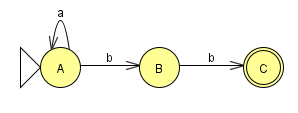
\includegraphics[width=0.4\textwidth]{img/graph4.png}
\end{center}
\noindent We can transform this finite state automaton into the following grammar using a known construction:

\begin{align*}
    A &\rightarrow aA | bB \\
    B &\rightarrow b
\end{align*}

\noindent Which can be simplified to : $A \rightarrow aA | bb$\\ \\
Now we find a finite automaton that corresponds to $ab^*ba$:
\begin{center}
    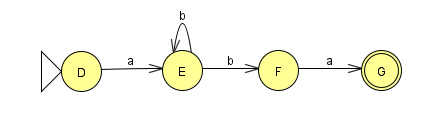
\includegraphics[width=0.5\textwidth]{img/graph5.png}
\end{center}
\noindent We easily derive the following regular grammar:
\begin{align*}
    D &\rightarrow aE \\
    E &\rightarrow bE | bF \\
    F &\rightarrow a
\end{align*}
\noindent That we simplify to:
\begin{align*}
    D &\rightarrow aE \\
    E &\rightarrow bE | ba
\end{align*} \\

\noindent Putting these grammars together we obtain:

\begin{align*}
    A &\rightarrow aA | bb \\
    D &\rightarrow aE \\
    E &\rightarrow bE | ba
\end{align*}

\noindent For simplicity and clarity, we rearrange and rename the symbols:

\begin{align*}
    S &\rightarrow A | aB \\
    A &\rightarrow aA | bb \\
    B &\rightarrow bB | ba
\end{align*}
